\documentclass[a4paper,12pt]{extarticle}
\usepackage[table,xcdraw]{xcolor}
\usepackage{pgfplots}
\usepackage[unicode, pdftex]{hyperref}
\usepackage[T2A]{fontenc}
\usepackage[utf8]{inputenc}
\usepackage[english,russian]{babel}
\usepackage{amsmath,amsfonts,amsthm, mathtools}
\usepackage{amssymb}
\usepackage{graphicx}
\graphicspath{{images/}}
\usepackage{wrapfig}
\usepackage{floatrow}
\usepackage{setspace}
\usepackage[headings]{fancyhdr}
\usepackage[margin=10pt,font={small,stretch=0,9},labelfont=bf,labelsep=period,
justification=centerlast]{caption}
\usepackage{array,tabularx,tabulary,booktabs}
\RequirePackage{multirow}
\RequirePackage{multicol}
\RequirePackage{longtable}
\usepackage{indentfirst}
\usepackage{hyperref}
\usepackage{icomma}
\newcommand*{\hm}[1]{#1\nobreak\discretionary{}
	{\hbox{$\mathsurround=0pt #1$}}{}}
\usepackage{soulutf8} 
\usepackage{etoolbox} 
\usepackage{geometry}
\geometry{top=20mm}
\geometry{bottom=20mm}
\geometry{left=20mm}
\geometry{right=20mm}
\DeclareMathOperator{\sgn}{\mathop{sgn}}
\usepackage[OT1]{fontenc}
\usepackage{amsmath}
\usepackage{amsfonts}
\usepackage{amssymb}
\usepackage{wasysym}
\usepackage{wrapfig}
\usepackage{physics}
\usepackage[normalem]{ulem}
\graphicspath{{pictures/}}
\DeclareGraphicsExtensions{.png,.jpg,.jpeg}
\usepackage{indentfirst}
\usepackage[T2A]{fontenc}
\usepackage{subfigure}
\usepackage{fancyhdr}
\usepackage{caption}

\usepackage{tabularx}
\usepackage{floatrow}
\usepackage{multicol}
\usepackage{lastpage}

\pgfplotsset{
  MyStyle1/.style={
    axis lines = middle,
    enlargelimits = true,
    grid=both,
    grid style={line width=.1pt, draw=gray!10},
    major grid style={line width=.2pt,draw=gray!50},
    minor tick num=5,
    enlargelimits=0.05,
    ticklabel style={font=\tiny,fill=white},
    xlabel style={at={(ticklabel* cs:1)},anchor=north west},
    ylabel style={at={(ticklabel* cs:1)},anchor=south east},
  }
}
\def\Slope{1.5}
\def\Intercept{-20}


% Настройка отчёркиваний и нумерации
\usepackage{fancyhdr}
\pagestyle{fancy}
\fancyhf{}

\fancyhead[L]{\nouppercase{\leftmark\hfill}}
\fancyfoot[RO, RE]{Страница \thepage \ из \pageref{LastPage}}
\renewcommand{\headrulewidth}{0.5pt}
\renewcommand{\footrulewidth}{0.5pt}

\usepackage{titlesec}
\titlelabel{\thetitle.\quad}

\pgfplotsset{compat=1.18}
\begin{document}

\thispagestyle{empty}
\begin{center}
	\textit{Федеральное государственное автономное образовательное\\ учреждение высшего образования }
	
	\vspace{0.5ex}
	
	\textbf{«Московский физико-технический институт\\ (национальный исследовательский университет)»}
\end{center}

\vspace{10ex}
\begin{figure}[!h]
  \begin{center}
    
\includegraphics[width = 0.8\textwidth]{MIPT.png}
  \end{center}
\end{figure}

\begin{center}
	
	\textbf{Лабораторная работа № 3.4.1}
	
	\vspace{1ex}
	
	по курсу общей физики
	
	на тему:
	
	\textbf{\textit{<<Диа- и парамагнетики>>}}
	
	\vspace{20ex}
	
	\begin{flushright}
		\noindent
		\textit{Работу выполнил:}\\  
		\textit{Легких Никита \\(группа Б05-301)}
	\end{flushright}
	\vfill
	Долгопрудный \\ \today
	\setcounter{page}{1}
\end{center}

\newpage

\textbf{Цель работы:}  измерение магнитной восприимчивости диа- и парамагнитного образцов.\\ \\
\textbf{В работе используются:} электромагнит, цифровые весы, милливеберметр, регулируемый источник постоянного тока, образцы.

\section*{Теоретическая справка}
В используемом нами методе Гюи требуется найти силу действующую на стержень вносимый в магнитное поле, она находится по формуле:
\begin{equation}
    F_x = \left( \frac{\partial W}{\partial x} \right)_I,
\end{equation}
частная производная магнитной энергии системы вдоль оси стержня при постоянном токе на обмотках электромагнита, то есть при постоянной магнитнойиндукции $B$

\begin{figure}[h]
    \begin{center}
    \begin{minipage}[h]{0.6\linewidth}
    Первоначально разделим стержень на три зоны:
    \begin{enumerate}
        \item I - в этой части будем считать что $B \approx 0$ и соответственно $dW_{\text{I}}\approx0$
        \item II - в этой зоне $B \approx const$ и соответственно энергия поля: $dW_{\text{II}} \approx \frac{B^2}{2 \mu \mu_0} \cdot dV$ для участка внутри стержня 
        \item III - в этой зоне $B \approx const$ и соответственно энергия поля: $dW_{\text{III}} \approx \frac{(\mu B)^2}{2 \mu_0} \cdot dV$ для участка вне стержня (тоже самое и для II) 
    \end{enumerate}
    Для подсчета $dW$ воспользуемся методов виртуальных перемещений и мысленно переместим стержень на $dx$ вниз и получим что 
    \begin{equation}
        dW = dW_{\text{I}} + dW_{\text{II}} + dW_{\text{III}} \approx (\mu - 1) \frac{(\mu B)^2}{2 \mu_0} S dx
    \end{equation}  
    \end{minipage}
    \hfill
    \begin{minipage}[h]{0.3\linewidth}
    
\includegraphics[width=1\linewidth]{3.4.1 Диа- и парамагнетики/стержень в поле магнита.png}
    \label{стержень в поле магнита}
    \end{minipage}
    \end{center}
\end{figure}
Получается что $\frac{dW}{dx} = (\mu - 1) \frac{B^2}{2 \mu_0} S = \chi \frac{B^2}{2 \mu_0} S$, где нашей целью как раз является определение коефициента $\chi$.
\begin{equation}
    F_x = \chi \frac{B^2}{2 \mu_0} S
\end{equation}
\newpage

\section*{Установка}
Схема установки изображена на рисунке ниже. Магнитное поле с максимальной индукцией 1.047 Тл создаётся в зазоре электромагнита, питаемого постоянным током. Диаметр полюсов существенно превосходит ширину зазора, поэтому поле в средней части зазора достаточно однородно. Величина тока, проходящего через обмотки электромагнита, задаётся регулируемым источником постоянного напряжения. 
\begin{figure}[h]
\centering
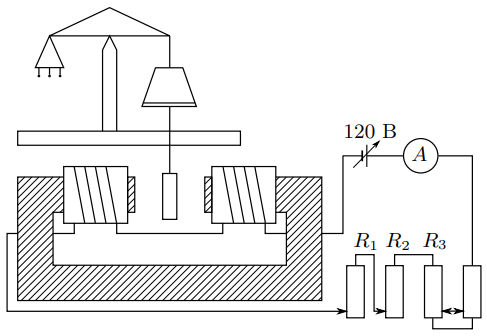
\includegraphics[width=0.5\linewidth]{схема установки}
\label{fig:mpr}
\end{figure} \\
Для определения коефициента восприимчивости будем определять "избыточную" силу  $\Delta F$, действующую на подвешиваемые нами стержни между обкладками, при пожаче тока на электромагнит. Избыточной она будет по сравнению с обычной силой тяжести.

\section*{Задание}
\begin{enumerate}
    \item Работа приборов проверена в соответствие с их документами. Приборная погрешность лабораторного источника: $\Delta I$ = 0,03 A и пределы изменения самой силы тока для нашей установки: 
    $$I_{\text{min}} = 0 \;\text{A},\;\; I_{\text{max}} = 1.17 \;\text{A}$$
    \item Проводим калибровку с помощью милливеберметра, его характеристики: 
    $$SN = 72\cdot10^{-4}\;\text{м}^2,\;\;\Delta \Phi = 0.1\;\text{мВб}$$
    Результаты калибровки: \\
    \begin{minipage}{0.3\textwidth}
    \begin{tabular}{|r|r|r|}
    \hline
    \multicolumn{1}{|l|}{$I,$  А} & \multicolumn{1}{l|}{$\Phi,$ мВб} & \multicolumn{1}{l|}{$B$, Тл} \\ \hline
    1.17                          & 7.3                              & 1.014                        \\ \hline
    1.05                          & 7.1                              & 0.986                        \\ \hline
    0.95                          & 6.6                              & 0.917                        \\ \hline
    0.85                          & 6.1                              & 0.847                        \\ \hline
    0.75                          & 5.4                              & 0.750                        \\ \hline
    0.66                          & 4.8                              & 0.667                        \\ \hline
    0.55                          & 4.0                              & 0.556                        \\ \hline
    0.45                          & 3.3                              & 0.458                        \\ \hline
    0.35                          & 2.6                              & 0.361                        \\ \hline
    0.25                          & 1.9                              & 0.264                        \\ \hline
    0.15                          & 1.1                              & 0.153                        \\ \hline
    0.10                          & 0.8                              & 0.111                        \\ \hline
    0.05                          & 0.4                              & 0.056                        \\ \hline
    \end{tabular}
    \end{minipage}
    \begin{minipage}{0.7\linewidth}
      \begin{tikzpicture}
        \begin{axis}[
          width=,
          height=,
          xlabel={$I,~\text{А}$},
          ylabel={$B,~\text{Тл}$},
          MyStyle1,
          ]
          \draw[red, domain=0:100] plot (\x,\Slope*\x+\Intercept);
          \addplot [only marks] plot [error bars/.cd,
                x dir=both, x fixed = 0.05,
                y dir=both, y explicit,
                      ] table [
                      x=I, y=B,
                x error minus=Ierr, x error plus=Ierr, y error minus=Berr, y error plus=Berr, col sep=comma] {calibrovka.csv};
        \end{axis}
      \end{tikzpicture}
    \end{minipage}
    \newpage
    \item Так как в нашем случае весы цифровые,они не требуют арретирования, их приборная погрешность в рамках наших измеренеий равна $\Delta m = 0,003$ г.
    \item Измеряем силы, действующие на алюминиевый образец в магнитном поле. Для этого, не включая электромагнит, подвесим к весам образец и измерим его массу, она равна $m_{\text{Al}} = (25,227\pm0.003)$ г. Теперь изменяя ток, пропускаемый через обмотки электромагнита меняем величину магнитной индукции и соответственно величину избыточной силы $\Delta P$ (далее просто $F$). \\ Результаты измерений:
    \begin{tabular}{|r|r|r|r|}
    \hline
    \multicolumn{1}{|l|}{$I$, А} & \multicolumn{1}{l|}{$m$, г} & \multicolumn{1}{l|}{$F$, мкН} & \multicolumn{1}{l|}{$\Delta F$, мкН} \\ \hline
    0.15 & 25.229 & 19.60  & 19.60 \\ \hline
    0.35 & 25.236 & 88.20  & 19.60 \\ \hline
    0.55 & 25.247 & 196.00 & 19.60 \\ \hline
    0.75 & 25.262 & 343.00 & 19.60 \\ \hline
    0.95 & 25.281 & 529.20 & 19.60 \\ \hline
    1.17 & 25.298 & 695.80 & 19.60 \\ \hline
    \end{tabular} \\
    Здесь $\Delta F = \mathcal{E}_m * F$
    \item Повторяем те же действия для других образцов c теми же пересчетами: \\
    Медный образец - $m_{\text{Cu}} = (83,070\pm0.003)$ г. \\
    Результаты измерений: 
    \begin{tabular}{|r|r|r|r|}
    \hline
    \multicolumn{1}{|l|}{$I$, А} & \multicolumn{1}{l|}{$m$, г} & \multicolumn{1}{l|}{$F$, мкН} & \multicolumn{1}{l|}{$\Delta F$, мкН} \\ \hline
    0.15 & 83.069 & -9.80   & 19.60 \\ \hline
    0.35 & 83.067 & -29.40  & 19.60 \\ \hline
    0.55 & 83.062 & -78.40  & 19.60 \\ \hline
    0.75 & 83.055 & -147.00 & 19.60 \\ \hline
    0.95 & 83.046 & -235.20 & 19.60 \\ \hline
    1.17 & 83.039 & -303.80 & 19.60 \\ \hline
    \end{tabular} \\ \\ \\
    Вольфрамовый образец - $m_{\text{W}} = (152,845\pm0.003)$ г. \\
    Результаты измерений: 
    \begin{tabular}{|r|r|r|r|}
    \hline
    \multicolumn{1}{|l|}{$I$, А} & \multicolumn{1}{l|}{$m$, г} & \multicolumn{1}{l|}{$F$, мкН} & \multicolumn{1}{l|}{$\Delta F$, мкН} \\ \hline
    0.15 & 152.906 & 597.80  & 19.60 \\ \hline
    0.35 & 152.932 & 852.60  & 19.60 \\ \hline
    0.55 & 152.965 & 1176.00 & 19.60 \\ \hline
    0.75 & 153.032 & 1832.60 & 19.60 \\ \hline
    0.95 & 153.098 & 2479.40 & 19.60 \\ \hline
    1.17 & 153.147 & 2959.60 & 19.60 \\ \hline
    \end{tabular} \\ \\ \\
    Образец С$_5$ - $m_{\text{C$_5$}} = (11,565\pm0.003)$ г. \\
    Результаты измерений: 
    \begin{tabular}{|r|r|r|r|}
    \hline
    \multicolumn{1}{|l|}{$I$, А} & \multicolumn{1}{l|}{$m$, г} & \multicolumn{1}{l|}{$F$, мкН} & \multicolumn{1}{l|}{$\Delta F$, мкН} \\ \hline
    0.15 & 11.591 & 254.80  & 19.60 \\ \hline
    0.35 & 11.648 & 813.40  & 19.60 \\ \hline
    0.55 & 11.711 & 1430.80 & 19.60 \\ \hline
    0.75 & 11.770 & 2009.00 & 19.60 \\ \hline
    0.95 & 11.819 & 2489.20 & 19.60 \\ \hline
    1.17 & 11.850 & 2793.00 & 19.60 \\ \hline
    \end{tabular} \\ \\ \\
\section*{Обработка результатов}
    \item см пункт 2
    \item Построим требуемые графики зависимости $|\Delta P| = |F| = f(B^2)$.\\
    Данные для графиков: \\ \\
    \begin{tabular}{|r|r|r|r|r|r|}
    \hline
    \multicolumn{1}{|l|}{$B^2$, Тл$^2$} & \multicolumn{1}{l|}{$\Delta B^2$, Тл$^2$} & \multicolumn{1}{l|}{$F_{\text{Al}}$, мкН} & \multicolumn{1}{|l|}{$F_{\text{Cu}}$, мкН} & \multicolumn{1}{l|}{$\Delta F$, мкН} \\ \hline
    0.02 & 0.03 & 19.60  & 9.80   & 19.60 \\ \hline
    0.13 & 0.07 & 88.20  & 29.40  & 19.60 \\ \hline
    0.31 & 0.11 & 196.00 & 78.40  & 19.60 \\ \hline
    0.56 & 0.15 & 343.00 & 147.00 & 19.60 \\ \hline
    0.84 & 0.18 & 529.20 & 235.20 & 19.60 \\ \hline
    1.03 & 0.20 & 695.80 & 303.80 & 19.60 \\ \hline
    \end{tabular} \\ \\
    \begin{minipage}{1\textwidth}
      \begin{tikzpicture}
        \begin{axis}[
          width=,
          height=,
          xlabel={$B^2,~\text{Тл$^2$}$},
          ylabel={$F,~\text{мкН}$},
          MyStyle1,
          ]
          \draw[blue, domain=0:100] plot (\x,654.1824533677143*\x-3.1312150387823863);
          \draw[red, domain=0:100] plot (\x,292.0293622242094*\x-6.727476137994188);
          \addplot [only marks] plot [error bars/.cd,
                x dir=both, x fixed = 0.05,
                y dir=both, y explicit,
                      ] table [
                      x=B2, y=Fal,
                x error minus=B2err, x error plus=B2err, y error minus=Ferr, y error plus=Ferr, col sep=comma] {f(B^2).csv};
          \addplot[purple, only marks] plot [error bars/.cd,
                x dir=both, x fixed = 0.05,
                y dir=both, y explicit,
                      ] table [
                      x=B2, y=Fcu,
                x error minus=B2err, x error plus=B2err, y error minus=Ferr, y error plus=Ferr, col sep=comma] {f(B^2).csv};
        \end{axis}
      \end{tikzpicture}
    \end{minipage}
    Черные точки с синей сглаживающей линией - Алюминий. \\ $k_{\text{Al}} = ( 654\pm19)$ мкН/Тл$^2$ \\
    Красные точки с красной сглаживающей линией - Медь. \\$-k_{\text{Cu}} = -(292\pm 9)$ мкН/Тл$^2$ \\ \\
    Здесь в соотвествии с формулой (3) $k = \chi \frac{S}{2 \mu_0}$ и тем фактом что $S = S_{\text{Cu}} = S_{\text{Al}} = \frac{\pi}{4} d^2$, где $d = 1$ см $\Rightarrow$ 
    $$\chi_{\text{Al}} = \frac{2 k_{\text{Al}} \mu_0}{S} = (2.06\pm0.06)\cdot 10^{-5}$$
    $$\chi_{\text{Cu}} = - \frac{2 k_{\text{Cu}} \mu_0}{S} = - (0.93\pm0.03)\cdot 10^{-5}$$
    Табличные значения: $\chi_{\text{Al}}^{\text{теор}} = 3.2\cdot 10^{-5}, \chi_{\text{Cu}}^{\text{теор}} = 0.92\cdot 10^{-5}$.

    \section*{Выводы}
    Нами были измерены магнитные восприимчивости алюминия и меди, причем с достаточно хорошей точностью вышло значение для меди:
    $$\mathcal{E}_{\text{Cu}} = 43\%$$ 
    $$\mathcal{E}_{\text{Al}} = 1\%$$
    Я считаю наш результат приемлемым, так как верный порядок величины найден везде.
\end{enumerate}


\end{document}